\chapter{Grundlagen}
In diesem Kapitel werden dem Leser die erforderlichen Grundkenntnisse für das Verständnis der vorliegenden Masterarbeit näher gebracht. \\




\section{Brain Computer Interface}

Ein \ac{BCI} ist eine Schnittstelle zwischen Gehirn und Computer, 
welche es ermöglicht Signale des Gehirns in verwertbare Informationen zu verwandeln.
Diese Informationen eröffnen dem zentralen Nervensystem, neben der neuromuskulären und der hormonellen, 
eine weitere Möglichkeit zur Kommunikation mit seiner Umwelt.

Dieser künstlich generierte Informationskanal kann genutzt werden, 
um verlorene oder eingeschränkte Fähigkeiten von Menschen mit motorischen Störungen in begrenzter Form wiederherzustellen.
Zusätzlich können diese Daten auch zur Verbesserung der Fähigkeiten gesunder Menschen beitragen \cite[S.3]{wolpaw2012braincomputer} 
oder in Abhängigkeit der gesammelten Daten könnte unterstützender Einfluss auf Hard- oder Software genommen werden.\\ \\
Die Aufzeichnung der Gehirnströme kann über invasive- oder nicht-invasive Methoden erfolgen.
Invasive Methoden zeichnen die Gehirnaktivität über Elektroden im Gehirn oder auf der Hirnhaut auf, 
während nicht-invasive Methoden die Signale indirekt über die Kopfhaut beziehen.
Die Messungen der Gehirnströme kann unter anderem über Magnetenze\-phalographie (\acs{MEG}), \ac{fMRT} oder \ac{EEG} \cite{berger2008braincomputer} erfolgen.

\pagebreak
\subsection{Elektroenzephalographie}
\vspace{0.3cm}
Die \acf{EEG} ist die am häufigsten verwendete Methodik zur Messung der Gehirnaktivität.
Bei ihr handelt es sich um eine nicht-invasive Messmethode wobei Elektroden auf der Kopfhaut platziert werden.
Für die Elektrodenplatzierung gibt es verschiedene international anerkannte Systeme, die je nach Anzahl und Position der Elektroden eine höhere Genauigkeit ermöglichen.
In Abbildung\footnote[1]{Bild-Quelle: \cite{Oostenvald2001}} \ref{electrodes} sind die Elektrodenpositionen gemäß des internationalen "`10-20-Systems"' \cite[S.370-375]{Jasp58} und des "`10-10-Systems"' dargestellt.
Die Kennzahl der Systeme gibt dabei Auskunft über den relativen Abstand der einzelnen Elektroden in Bezug zu Referenzpunkten auf der Kopfoberfläche.\\


\begin{figure}[h!]
\begin{center}
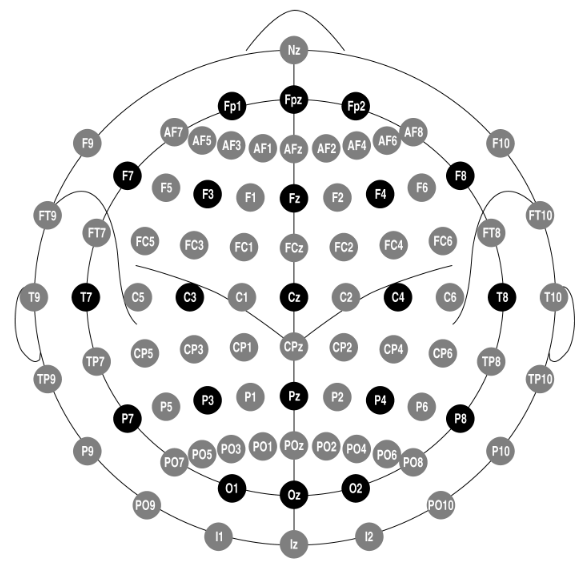
\includegraphics[scale=0.61]{images/1010.png}
\caption{Die Elektrodenpositionen des internationalen 10-20-Systems (schwarz) und des 10-10-Systems (schwarz und grau)}
\label{electrodes}
\end{center}
\end{figure}


Die Verwendung von \acs{EEG}'s ist deshalb vorteilhaft, da sie relativ kostengünstig und einfach einzusetzen sind.
Medizinische \acs{EEG}'s befinden sich überwiegend in speziell abgeschotteten Räumen, jedoch gibt es auch einfache zu handhabende tragbare Geräte, sodass eine hohe Verfügbarkeit besteht.
Allerdings existieren neben den Vorteilen auch Nachteile, da die Auflösung und Frequenzreichweite begrenzt ist und Artefakte durch Muskelaktivität oder Augenblinzeln entstehen können \cite{Graimann2010}.









\subsection{Oddball-Paradigma}
\vspace{0.3cm}

Das Oddball-Paradigma oder auch Zwei-Reiz-Diskriminationsparadigma \cite[S.9]{paehge2006verschiedenen} genannt, 
beschreibt eine besondere Charakteristik von Stimulus-Ereignissen, die in zwei Klassen unterteilt werden können.
Dabei existiert eine Klasse von häufigen und eine Klasse von seltenen Ereignissen. 
Jedes der seltenen und damit unerwarteten Ereignisse ist ein "`Oddball-Ereignis"'.\\



\subsection{P300 Ereigniskorreliertes Potential}
\vspace{0.3cm}

Im Zusammenhang mit einem "`Oddball-Ereignis"' steht in der Regel ein ereigniskorelliertes positives Potential.
Es tritt etwa 300ms nach dem auslösenden Ereignis auf. 
Die Latenzzeit kann jedoch zwischen 250ms und 750ms variieren, was von der nicht notwendigerweise bewussten Entscheidung abhängt, ob das Ereignis aufgetreten ist.\\

\begin{figure}[h!]
\begin{center}
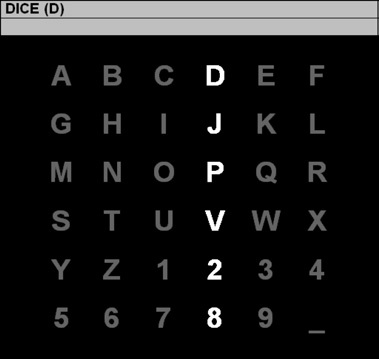
\includegraphics[scale=0.6]{images/P300Speller.jpg}
\caption{Die 6x6 Matrix eines P300 Spellers mit hervorgehobener Spalte}
\label{P300Speller}
\end{center}
\end{figure}

Basierend auf diesem \ac{P300 ERP} wurde 1988 von Farwell und Donchin \cite{FarwellDonchin1988} ein sogenannter \textit{"`P300 Speller"'} eingeführt. 
Dabei werden die Stimuli als Zeilen und Spalten einer Matrix zusammengefasst. 
Die Zeilen und Spalten der Matrix werden hierbei in zufälliger Reihenfolge kurz sichtbar hervorgehoben, wie in Abbildung\footnote[1]{Bild-Quelle: \cite[S.300]{P300SpellerCompare}} \ref{P300Speller} zu sehen ist. 
Der Benutzer sollte sich während dieser Prozedur auf das auszuwählende Feld konzentrieren. 
Sobald die Zeile bzw. Spalte des Zielfelds aufblitzt, wird ein \acs{P300 ERP} evoziert. 
Das Zielfeld ergibt sich anschließend aus Kombination der Zeilen und Spalten, die ein \acs{P300 ERP} ausgelöst haben.
Durch dieses Vorgehen ist es möglich für viele verschiedene Anwendungsmöglichkeiten "`Ja/Nein"'- bzw. "`Ziel/Nicht-Ziel"'-Antworten zu ermitteln.
Dieses Prinzip funktioniert bei allen Experimenten deren Ereignisse dem Oddball-Paradigma folgen \cite[S.215ff]{wolpaw2012braincomputer}.\\



\subsection{Emotiv EPOC}
\vspace{0.3cm}

Das Emotiv EPOC \cite{Emotiv2014} in Abbildung \ref{EmotivEPOC} ist ein für praktische Anwendungen entwickeltes, hochauflösendes und portables \acs{BCI}.
Es verwendet für die \acs{EEG}-Signalerfassung 16 Kanäle, wovon 2 als Referenz dienen.
Die Elektroden des Emotiv EPOC werden gemäß des internationalen "`10-20-System"' \cite[S.370-375]{Jasp58} an den Positionen 
AF3, F7, F3, FC5, T7, P7, O1, O2, P8, T8, FC6, F4, F8, AF4 platziert (Zu sehen in Abbildung\footnote[1]{Bilder-Quelle: \cite{Emotiv2014}}
\ref{EmotivMAP}). 
Die Genauigkeit kann allerdings durch individuelle Faktoren wie die Kopfgröße negativ beeinflusst werden, da die Elektrodenplatzierung des Emotiv EPOC auf eine Größe genormt ist.\\

\begin{figure}[ht]
\centering
\begin{minipage}[b]{0.45\linewidth}	
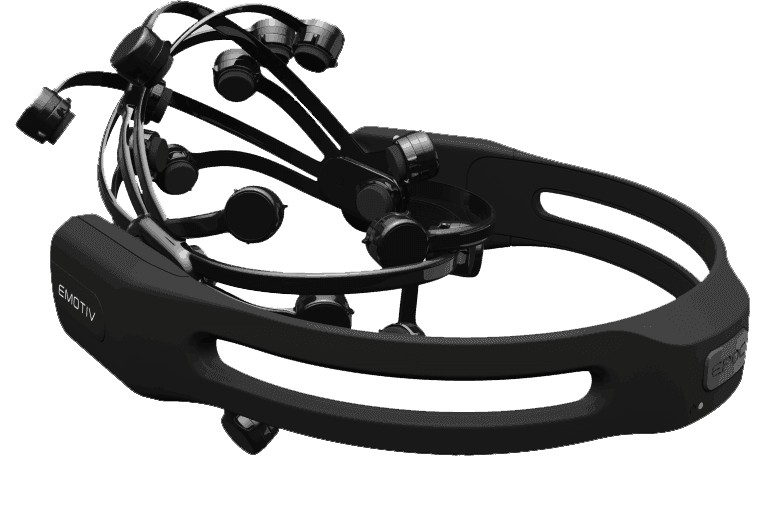
\includegraphics[scale=0.3]{images/emotivEpoc.png}
\caption{Das Emotiv EPOC \acs{BCI}}
\label{EmotivEPOC}
\end{minipage}
\quad
\begin{minipage}[b]{0.45\linewidth}
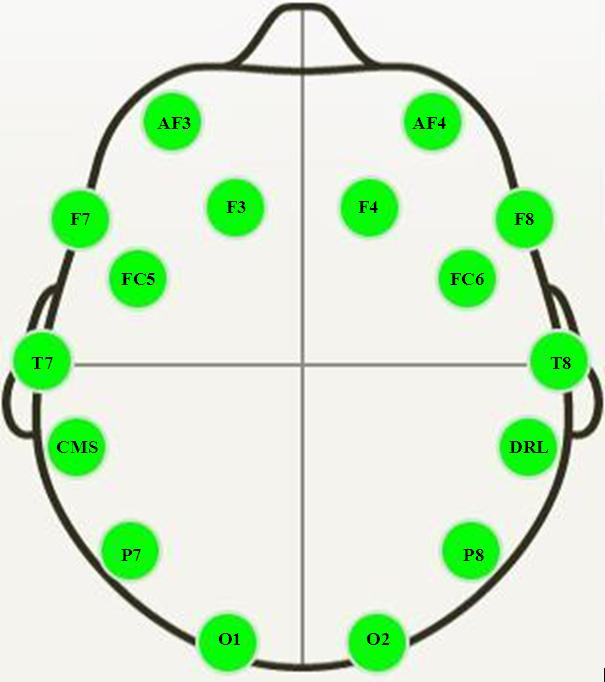
\includegraphics[scale=0.3]{images/emotivMap.jpg}
\caption{Die Elektroden des Emotiv EPOC}
\label{EmotivMAP}
\end{minipage}
\end{figure}








\pagebreak
\section{BCI2000}
\label{BCI2000}
Bei \acs{BCI2000} handelt es sich um eine quelloffene Software Plattform zur Verwendung von Brain-Computer-Interfaces. 
Sie wurde entwickelt, um ein leistungsfähiges und einfach zu erweiterndes \acs{BCI} Forschungs-Framework bereitzustellen.
Das Framework stellt viele Module zur Signalerfassung, -bearbeitung und -verwertung zur Verfügung. 
Insbesondere gibt es für viele \acs{BCI}'s entsprechende Module zur Signalerfassung.

Damit die Echtzeiterfassung der Daten gewährleistet werden kann, ist die Platform in C++ geschrieben.
Die Programmstruktur ist modular,
wie in Abbildung\footnote[1]{Bild-Quelle: \cite[S.39]{schalk2010practical}} \ref{BCI2000Design},
aus vier Teilen zusammengesetzt.
Das \textit{Operator}-Modul ist hierbei das Herzstück der Platform und je nach Notwendigkeit können die drei anderen Module ausgetauscht oder erweitert werden.\\

\begin{figure}[h!]
\begin{center}
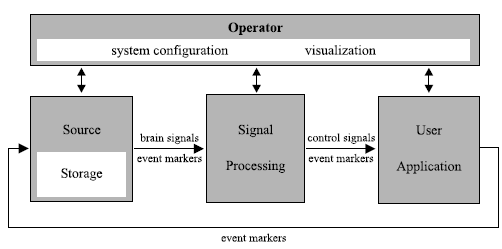
\includegraphics[scale=1]{images/BCI2000Design.png}
\caption{Eine vereinfachte Darstellung des Designs der \acs{BCI2000} Platform.}
\label{BCI2000Design}
\end{center}
\end{figure}

\begin{itemize}
\item Das \textit{Operator}-Modul: Dieses Modul steuert das Zusammenwirken aller vier Module.
\item Das \textit{Source}-Modul: Dieses Modul bezieht die \acs{EEG}-Signale und reicht sie an das \textit{Signal-Processing}-Modul weiter.
\item Das \textit{Signal-Processing}-Modul: Dieses Modul verarbeitet die erhaltenen Sig\-nale, extrahiert Merkmale und leitet diese als verwertbare Befehle weiter.
\item Das \textit{User-Application}-Modul: Dieses Modul empfängt die Befehle des \textit{Signal-Processing}-Modules
und benutzt diese zur Steuerung der Applikation oder des zugrunde liegenden Geräts. Des Weiteren steuert es die Präsentation der Stimuli und markiert diese im \textit{Source}-Modul, 
so dass eine Assoziation zwischen Stimuli und Signal möglich ist. \\
\end{itemize}

Die Architektur des \acs{BCI2000} ist so konzipiert, dass immer alle vier Module nacheinander ausgeführt werden müssen. 
Dabei fungiert das \textit{Operator}-Modul gewissermaßen als Server, bei dem sich die anderen drei Funktionsmodule anmelden. 
Die Interprozesskommunikation zwischen den vier Modulen geschieht mittels einem auf TCP/IP basierenden Protokolls \cite[s.38ff]{schalk2010practical},
worüber Signal- und Steuerinformationen, sowie globale Zustandvariablen kommuniziert werden können.
Die in der Abbildung dargestellten "`event markers"' zwischen dem \textit{User-Application}-Modul und dem \textit{\mbox{Source}}-Modul sind in diesem Zusammenhang besonders wichtig, 
da diese mit Hilfe einer Assoziationskarte die Zuordnung der einzelnen Stimuli und korrespondierender \acs{P300 ERP} ermöglichen.\\




\pagebreak
\section{Point\&Click}
Bei "`Point\&Click"' handelt es sich um ein Computerspiel-Genre, deren Spiele üblicherweise dem Eingabeparadigma der alleinigen Maussteuerung folgen \cite[Kapitel 11]{darby2013creating}.
Diese häufig auch "`Point\&Click-Adventures"' genannten Spiele, 
versetzen den Spieler in eine meist fiktive Welt und führen ihn durch eine dazugehörige Geschichte ein.
Solche Welten werden oft als einzelne Szenen oder Räume dargestellt, aber auch eine kontinuierliche Darstellung ist möglich.
Eine Szene ist für gewöhnlich ein Zimmer in einem Haus oder eine Landschaft in der Objekte, Charakter und Ereignisse integriert sind. 
Der Spieler erkundet die Szenen in aller Regel und muss oftmals Rätsel lösen, um im Spielfortschritt weiter voranzuschreiten.
Mit der Maus werden deshalb die zur Verfügung stehenden Aktionen ausgewählt, um anschießend das Ziel für diese zu bestimmen.\\
Gut durchdachte Spiele dieses Genre können durch ihre Rätsel sehr herausfordernd sein und die Aufmerksamkeit eines Spielers fördern.
Da bei klassischen Point\&Click-Spielen jedoch keine kontinuierliche Steuerung erfolgt, sind diese im allgemeinen langsamer als andere Spiele.
Einer der bekanntesten Ableger dieses Genres ist unter anderem die von LucasArts entwickelte "`The Secret of Monkey Island"'-Reihe von 1990, 
dargestellt in Abbildung\footnote[1]{Bild-Quelle: \cite{TSOMI90} } \ref{MonkeyIsland}. \\


\begin{figure}[h!]
\begin{center}

\includegraphics[scale=0.7]{images/monkeyIsland.png}
\caption{Eine Szene aus "`The Secret of Monkey Island"'}
\label{MonkeyIsland}
\end{center}
\end{figure}


\pagebreak
\section{Adventure Game Studio}
Das \ac{AGS}\footnote{Quelle: \cite{AGS2014}} 
ist eine quelloffene Point\&Click Spiele Engine, 
die in C++ geschrieben wurde und aus der eigentlichen Engine und einem dazugehörigen Editor besteht.
Zu Beginn dieser Masterarbeit lag die Engine in der Version 3.3 vor.
Sie besitzt eine umfangreiche Dokumentation und verfügt über ein Plugin-System zur einfachen Erweiterung der Engine und des Editors.
Das \acs{AGS} entwickelt sich, dank einer großen Gemeinschaft aus Engine- und Spieleentwicklern, kontinuierlich weiter.
Zudem existiert eine Vielzahl an Nutzern der daraus entstandenen Spiele.
Mit \acs{AGS} ist es möglich einfache Point\&Click-Adventures für Windows zu erstellen.
Eine Unterstützung für andere Betriebssysteme wie Linux oder MacOS soll es in zukünftigen Versionen geben.\\

Die Erstellung der Point\&Click-Adventures erfolgt im dazugehörigen Editor, einer einfach gehaltenen Entwicklungsumgebung, dessen Skript-Sprache auf Microsofts .NET Framework basiert.
Der Editor ermöglicht es Räume, Spielfiguren, Sounds und Grafiken innerhalb der Spiele zu erstellen und zu integrieren. 
Mit der integrierten Skript-Sprache können verschiedene Ereignisse ausgelöst und behandelt werden, um dem Spiel eine gewisse Dynamik zu verleihen.
Die Benutzeroberfläche eines Spiels kann vom Entwickler komplett individuell erstellt und auf die jeweiligen Bedürfnisse eines Spiels oder der Spieler angepasst werden.
Der Benutzer des Editors muss sich bei der Entwicklung eines Spiels keine Gedanken um Wegfindung oder Kameraführung machen.
Ebenso stellt die Engine Funktionen wie das Speichern und Laden von Spielständen bereit.
Diese müssen lediglich unter Verwendung der entsprechenden Befehle in die \ac{GUI} des Spiels integriert werden. \\























